\documentclass[a4paper,12pt]{article}

\usepackage[utf8]{inputenc}
\usepackage[italian]{babel}
\usepackage{amsmath}
\usepackage{geometry}
\usepackage{listings}
\usepackage{hyperref}
\usepackage{graphicx}
\usepackage{booktabs}
\usepackage{caption}
\usepackage{subcaption}
\usepackage{float}

\geometry{margin=2.5cm}

\graphicspath{{./}}

\lstset{
    basicstyle=\ttfamily\small,
    breaklines=true,
    frame=single,
    numbers=left,
    numberstyle=\tiny,
    xleftmargin=1.5em
}

\title{Relazione Laboratorio HPC -- Esercitazione 2}
\author{Federico Becchi}
\date{}

\begin{document}

\maketitle
\tableofcontents
\newpage

% =========================================================
\section{Obiettivo}

Obiettivo di questa relazione \`e eseguire programmi di benchmark e visualizzarne i risultati.

% =========================================================
\section{Timing}

Obiettivo di \texttt{timing.c} \`e quello di calcolare il tempo di esecuzione e il tempo di CPU.

\subsection{Risultati PC}

\begin{lstlisting}[language=bash]
#!/bin/sh

gcc timing.c -o timing -O2

./timing > timing_pc.csv
\end{lstlisting}

\begin{figure}[H]
\centering
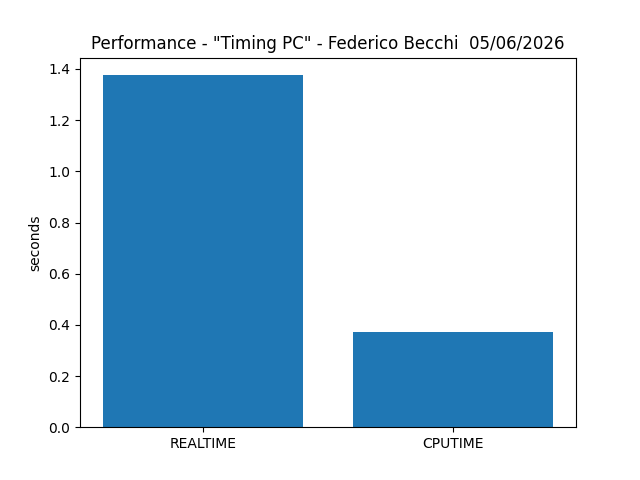
\includegraphics[width=0.75\textwidth]{../timing/timing_PC.png}
\caption{Risultati timing -- PC.}
\end{figure}

\subsection{Risultati Cluster}

\begin{figure}[H]
\centering
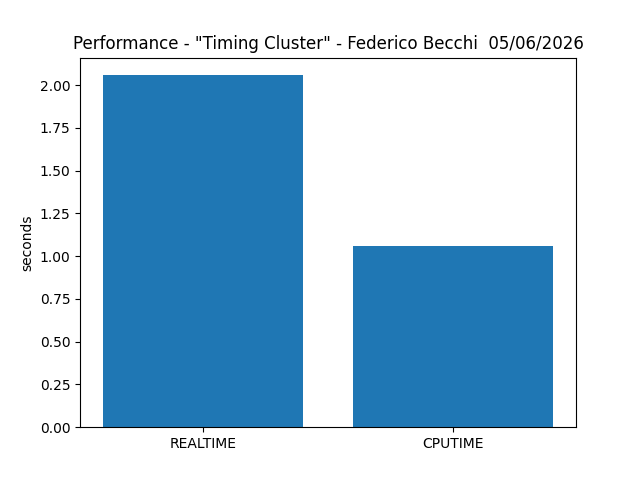
\includegraphics[width=0.75\textwidth]{../timing/timing_cluster.png}
\caption{Risultati timing -- Cluster.}
\end{figure}

\begin{figure}[H]
\centering
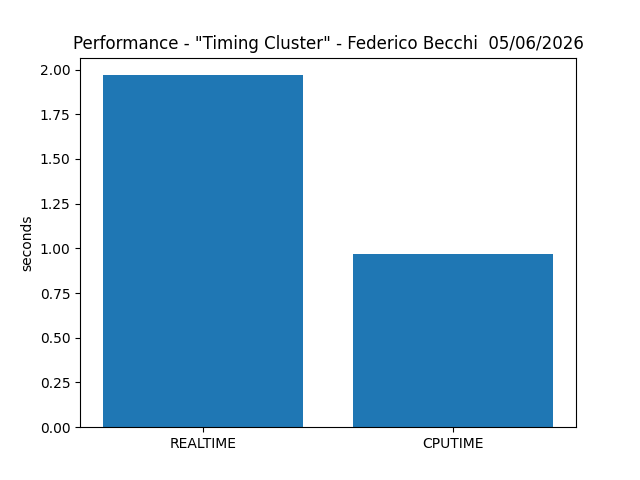
\includegraphics[width=0.75\textwidth]{../timing/timing.png}
\caption{Confronto risultati timing.}
\end{figure}

% =========================================================
\section{Matrix Mul}

\subsection{Cosa fa}

Obiettivo \`e misurare le performance espresse in FLOP/S della moltiplicazione tra due matrici. Il numero di operazioni FP \`e
\[
\text{flops} = 2n^3
\]
con $n$ la lunghezza del lato delle matrici quadrate ($n \times n$).

\subsubsection{mm.c}

Due modalit\`a di esecuzione:
\begin{itemize}
    \item \textbf{naive}: tripla loop naive di \texttt{for}
    \item \textbf{-g}: opzione \texttt{gsl\_blas\_sgemm}
\end{itemize}

\subsubsection{Cosa fa omp\_mm.c}

Versione parallelizzata di \texttt{mm.c} usando OpenMP. La parallelizzazione su pi\`u thread avviene sia per la moltiplicazione sia per l'inizializzazione.

\subsection{CPU}

\subsubsection{mm.slurm}

Compila \texttt{mm.c} con gcc e con Intel, con alcune opzioni di compilazione, ed esegue sia Naive che GS.

\subsubsection{omp\_mm\_scaling.slurm}

Esegue \texttt{open\_mm.c} con 1024 (o 2048) come $n$ (lato di una matrice) e 1, 2, 4, 8 thread.

\subsection{GPU}

\subsubsection{matrixMul.slurm}

Esegue il benchmark della moltiplicazione matriciale sulla GPU con dimensione matrice 1024.

Valori csv prima del convertimento:
\begin{lstlisting}
Performance= 2132.57 GFlop/s, Time= 1.007 msec, Size= 2147483648 Ops, WorkgroupSize= 1024 threads/block
\end{lstlisting}

Valori csv dopo il convertimento:
\begin{lstlisting}
1024, 2.14748, 0.001007, 2132.57, "", ""
\end{lstlisting}

\subsection{Plotting}

\begin{figure}[H]
\centering

\includegraphics[width=0.75\textwidth]{../matrixMul/PLOTTING/Cluster/matrixMul.png}
\caption{Prestazioni moltiplicazione matriciale -- Cluster.}
\end{figure}

% =========================================================
\section{Band-latency}

\subsection{Band}

\begin{itemize}
    \item \textbf{band1}: bandwidth con 2 task sullo stesso nodo
    \item \textbf{band2}: bandwidth con 1 task per nodo
\end{itemize}

\subsection{Latency}

\begin{itemize}
    \item \textbf{lat1}: latenza intra-nodo
    \item \textbf{lat2}: latenza inter-nodo
\end{itemize}

Risultati dentro band e lat.

\begin{figure}[H]
\centering
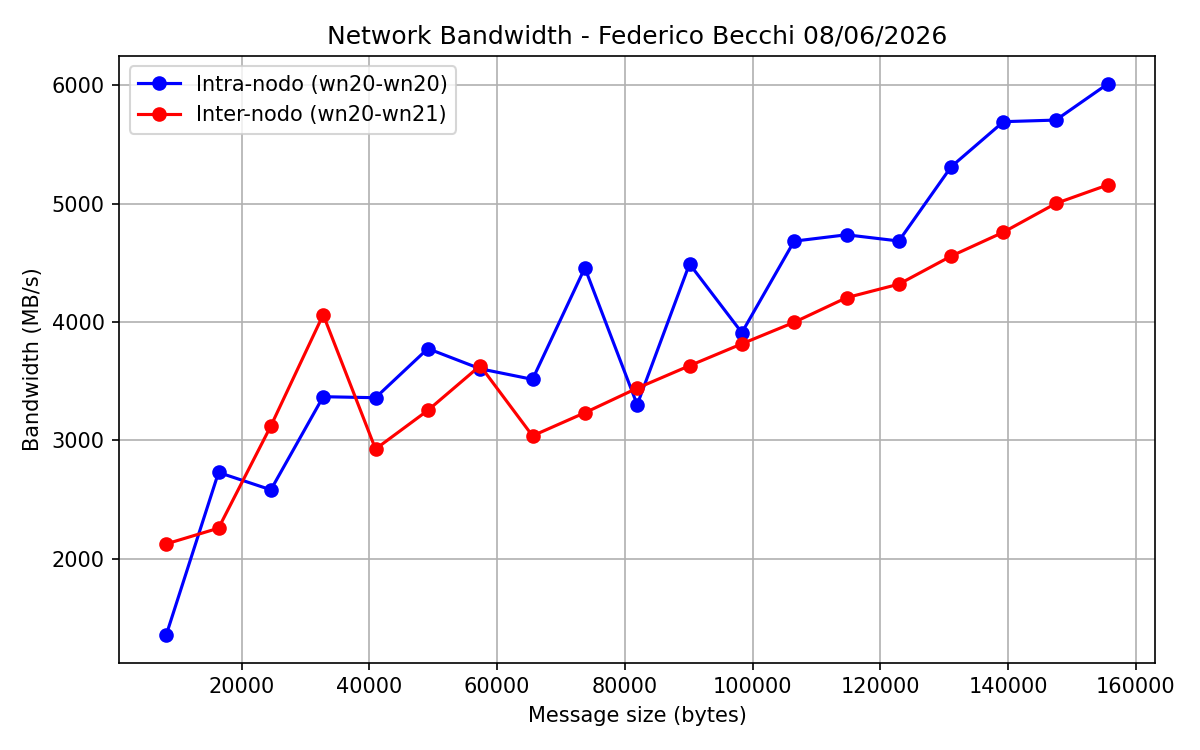
\includegraphics[width=0.75\textwidth]{../network/results/Cluster/band.png}
\caption{Risultati bandwidth.}
\end{figure}

\begin{figure}[H]
\centering
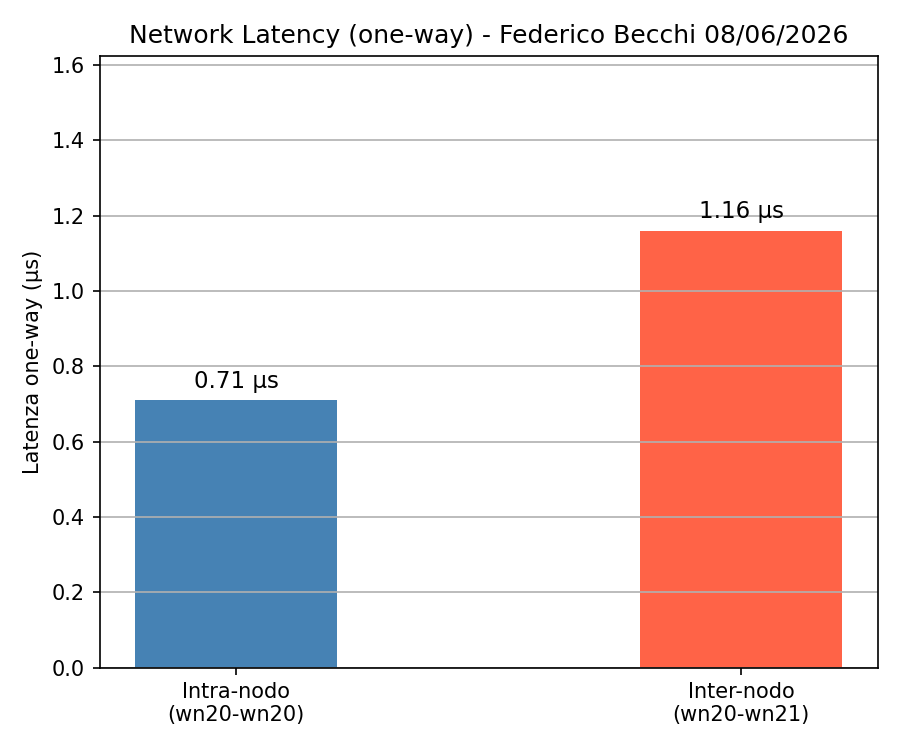
\includegraphics[width=0.75\textwidth]{../network/results/Cluster/lat.png}
\caption{Risultati latenza.}
\end{figure}

% =========================================================
\section{Disktest}

PC benchmark usando \texttt{dd}: scrittura di 512 MB in 512 blocchi, lettura dello stesso file appena scritto.

\subsection{Results PC}

\begin{lstlisting}
Working directory: /Users/federicobecchi/Documents/HPC/lab/02/storage
Free space: /dev/disk3s5   460Gi   341Gi    95Gi    79%    2.5M  1.0G    0%   /System/Volumes/Data
Write to file:
512+0 records in
512+0 records out
536870912 bytes transferred in 0.557984 secs (962161840 bytes/sec)

Read from file:
512+0 records in
512+0 records out
536870912 bytes transferred in 0.149935 secs (3580691046 bytes/sec)
\end{lstlisting}

\subsection{Cluster}

Stesso test di prima ma eseguito su \texttt{\$HOME}, \texttt{\$SCRATCH}, \texttt{\$ARCHIVE}.

\subsection{Results Cluster}

\begin{lstlisting}
/var/spool/slurm/slurmd/job2485102/slurm_script: line 2: BATCH: command not found
####################################
Running in: /hpc/home/federico.becchi
---- disktest output ----
Write to file:
2048+0 records in
2048+0 records out
2147483648 bytes (2.1 GB) copied, 7.06106 s, 304 MB/s

Read from file:
2048+0 records in
2048+0 records out
2147483648 bytes (2.1 GB) copied, 0.631048 s, 3.4 GB/s
------------------------
####################################
Running in: /hpc/scratch/federico.becchi
---- disktest output ----
Write to file:
2048+0 records in
2048+0 records out
2147483648 bytes (2.1 GB) copied, 2.42872 s, 884 MB/s

Read from file:
2048+0 records in
2048+0 records out
2147483648 bytes (2.1 GB) copied, 0.856719 s, 2.5 GB/s
------------------------
ARCHIVE not defined, skipping
####################################
JOB FINISHED
\end{lstlisting}

\end{document}
